\section*{Analisi \emph{RFLP} di polimorfismi a singolo nucleotide}

	\subsection*{Introduzione}
	Questo esperimento valuta la variabilità genetica dovuta a singoli polimorfismi di singoli nucleotidi (\emph{SNPs}). 
	Per \emph{SNPs} si intende una variazione genetica e rappresenta un cambio di nucleotide all'interno della nostra sequenza. 
	In linea di massima gli \emph{SNPs} possono essere visti come delle mutazioni dato che sono comunque una variazione nella sequenza, ma a cambiare è la presenza con cui si presentano nella popolazione. 
	Le mutazioni, infatti, sono molto più rare  rispetto agli \emph{SNPs} che si trovano in almeno nell'$1\%$ della popolazione. 
	Inoltre, gli \emph{SNPs} non sono sempre associati a delle patologie, infatti, nella maggior parte dei casi vanno a determinare alcune nostre caratteristiche. 
	Durante questa esperimento si è andati a valutare la capacità di una persona di percepire più o meno il gusto dell'amaro tramite lo studio del recettore \emph{TAS2R38}.
		
		\subsubsection*{Recettore \emph{TAS2R38}}
		Questo recettore è in grado di andare a percepire i glucosinolati che sono dei composti presenti in alcuni alimenti che mangiamo, come i broccoli. 
		\emph{TAS2R38} si trova sul cromosoma $7$ e al suo interno presenta cinque differenti polimorfismi, ma i tre più comuni si trovano in determinate posizioni della proteina all'aminoacido $49$, $263$ e $296$. 
		Questi tre polimorfismi danno origine a due fenotipi, ma a tre aplotipi:
		\begin{multicols}{2}
		\begin{itemize}
			\item Taster con aplotipo \emph{PAV}.
			\item Taster con aplotipo \emph{AVV} sono meno frequenti ($3\%$), ma hanno la stessa capacità di percepire il gusto di quelli che vengono considerati taster più frequenti.
			\item Non-taster con aplotipo \emph{AVI}. 
		\end{itemize}
		\end{multicols}
    
		\subsubsection*{Procedimento}
		Per verificare la presenza di \emph{SNPs} è stata amplificata una porzione del gene \emph{TAS2R38} mediante una \emph{PCR}.
		Per andare a discriminare i diversi genotipi si è deciso di utilizzare un enzima di restrizione (\emph{Fun4H1}). 
		Si sono caricate le \emph{PCR} digerite con enzimi di restrizione e sotto ciascuna di queste è stata caricata la \emph{PCR} non digerita. 
		Per poter visualizzare meglio i risultati è stato aggiunto anche un colorante blu. 
	   
		\subsubsection*{Risultati aspettati}
		Dalla \emph{PCR} non digerita con enzima di restrizione non ci si aspetta di avere alcuna indicazione su variazioni a livello nucleotidico. 
		Nelle \emph{PCR} digerite con enzimi di restrizione, invece, ci si aspetta di vedere alcune differenze. 
		Se tutti i cinque siti di restrizione sono integri ci si aspetta un determinato tipo di bandeggio, mentre se in alcuni casi l'enzima di restrizione non riuscisse a riconoscere il sito di restrizione quello che si nota è un bandeggio completamente differente. 
		Ci si aspetta che si presentino tutte e tre le condizioni, dato che i campioni che abbiamo provengono da tre individui con diverso aplotipo. 
		Dopo la corsa su gel di agarosio si riesce ad osservare che:
		\begin{itemize}
			\item Il taster \emph{PAV} presenta le bande più basse.
			\item Il non taster \emph{AVI} presenta le bande più alte.
			\item Il taster meno frequente \emph{AVV} presenta entrambe le componenti. 
		\end{itemize}
	
	\subsection*{Risultati}
	\begin{figure}[H]
		\centering
		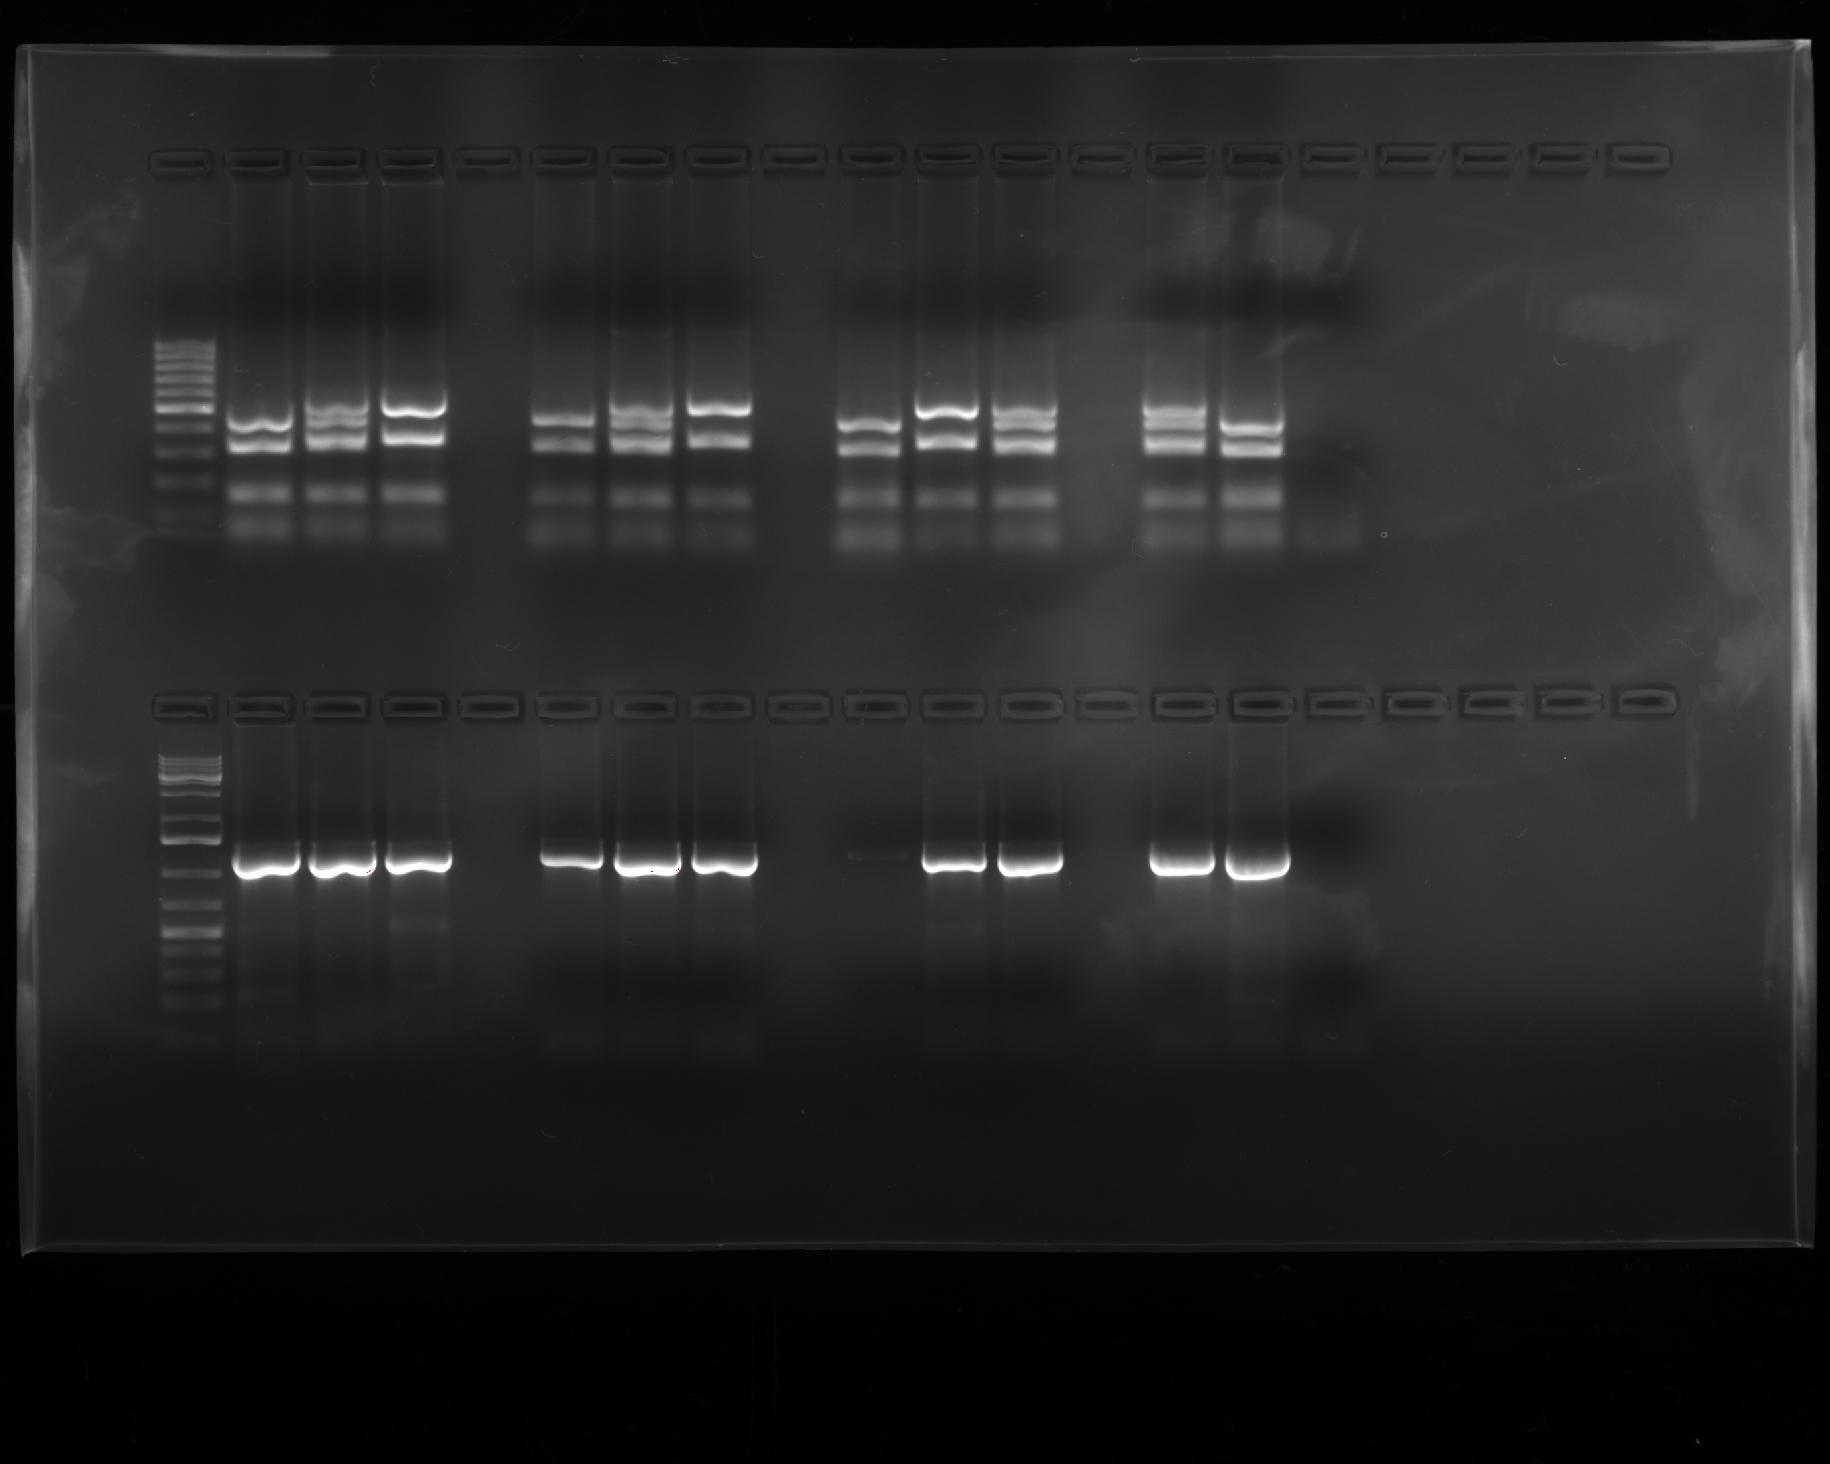
\includegraphics[width=\textwidth]{./Pics/RFLP/RFLP_gruppoD.jpg}
		\caption{Elettroforesi su gel d'agarosio dei risultati della \emph{PCR}}
		\label{fig10}
	\end{figure}

	\subsection*{Considerazioni finali}
	Facendo riferimento agli ultimi due gruppi (figura~\ref{fig10}) si possono fare alcune considerazioni finali su la riuscita o meno dell'esperienza. 
	Come previsto, dalla \emph{PCR} non digerita non si ha avuto alcuna indicazione sulle variazioni a livello nucleotidico.
	Per quanto riguarda il primo dei due gruppi si può dire che l'esperienza è avvenuta con successo, in quanto si sono ottenuti i risultati attesi. 
	Unica nota va fatta sulla corsa del DNA dell'individuo taster in quanto era presente meno colorante. 
	Per quanto riguarda il secondo gruppo non ci sono stati problemi per l'individuo taster e l'individuo taster meno frequente, ma purtroppo non si è potuta apprezzare la corsa del non taster. 
	Per entrambi si può comunque concludere che l'aplotipo \emph{AVV} ha la componente di entrambi e per questo motivo è considerato eterozigote.
